%
% fig-fundamental.tex
%
% (c) 2026 Prof Dr Andreas Müller
%
\begin{figure}
\centering
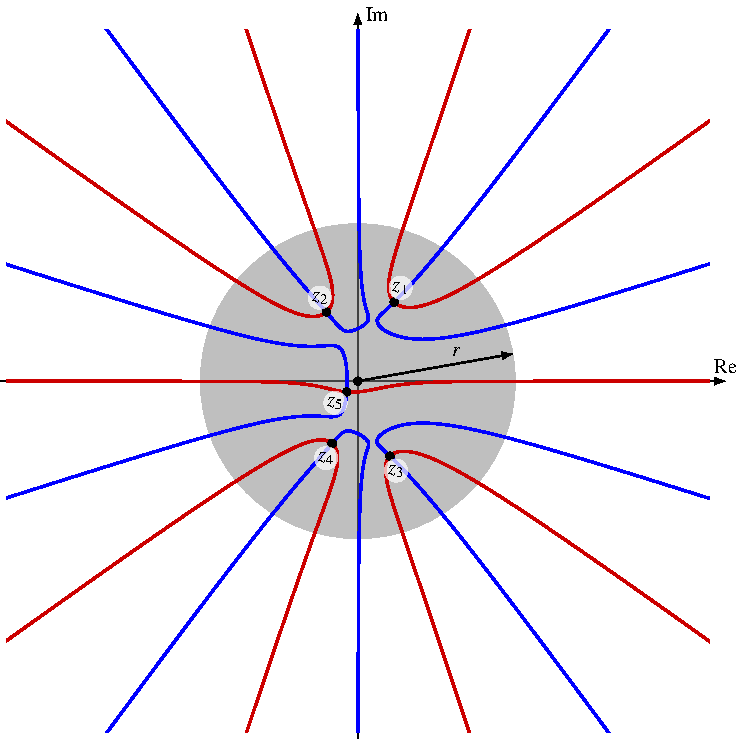
\includegraphics{chapters/010-komplex/images/fundamental.pdf}
\caption{Illustration von Gauss' Idee zum Beweis des Fundamentalsatzes
der Algebra anhand eines Polynoms $p(z)$ vom Grad 5.
Die roten Linien bestehen aus den Punkten $z$, für die der
Imaginärteil $\operatorname{Im} p(z)$ verschwindet.
Auf den blauen Kurven verschwindet der Realteil $\operatorname{Re}p(z)$.
Es kann höchstens 5 rote und blaue Kurven geben.
Ein grosser Kreis um den Nullpunkt schneidet abwechslungsweise rote und
blaue Kurven insgesamt je 10 mal.
Also müssen sich diese Kurven im Inneren des grauen Kreises schneiden.
Die Schnittpunkte sind Nullstellen $z_k$ des Polynoms
\label{buch:komplex:fig:fundamental}}
\end{figure}
